%%%% PROCESAR con PdfLaTeX !!!!!


\documentclass[12pt]{book}++
\usepackage{geometry}\geometry{top=2cm,bottom=2cm,left=3cm,right=3cm}
\usepackage{amssymb}
\usepackage{amsmath}
\usepackage{graphicx}
\usepackage{txfonts}




\begin{document}
\thispagestyle{empty}

\begin {center}

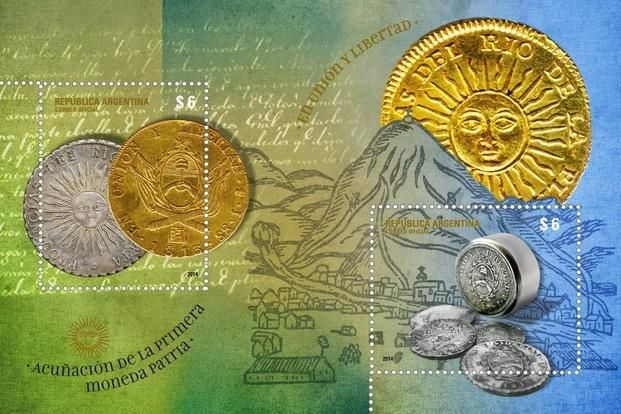
\includegraphics[scale=.4]{1484058646033.jpg}

\medskip
UNIVERSIDAD DE BUENOS AIRES

Facultad de Econom\'ia


\vspace{3cm}


\textbf{\large HISTORIA ECONOMICA SOCIAL GENERAL}

\vspace{2cm}


Este es un compendio de apuntes de clase, resumenes de la bibliograf\'ia obligatoria y es un aporte para los alumnos y los interesados en general.
De ninguna man\'era pretende ser una gu\'ia de estudio, ni remplaza las clases presenciales, el material oficial de la catedra esta disponible en el web site de la m\'ateria.
\\

\end {center}


\vspace{2.5cm}

\noindent Autor:\,	Isaac Edgar Camacho Ocampo
 
\noindent Carrera:\,	Licenciado en Econom\'ia

\vspace{1cm}

\vspace{1cm}

\noindent Buenos Aires, 2019

\newpage


\tableofcontents

\tableofcontents
\chapter{Revoluci\'on industrial}
\section{¿En que consistio la revolucion industrial?}
Capitulo 3,5 del libro de Barbero
 Comenzaremos con la siguiente interrogante ¿cual es el significado que los historiadores le atribuyen hoy al termino RI? Como vimos anteriormente no existe un consenzo entre los diferentes autores.
 \\
\\
\textbf{David landes propone 3 definiciones}
\begin{itemize}
 \item \textbf{revolucion industrial} en minuscula, se refiere al complejo de innovaciones tecnol\'ogicas que al sustituir la habilidad humana por maquinaria y la fuerza humana y animal por energ\'ia mec\'anica, provoca el paso desde un tipo de producci\'on artesanal a un tipo de producci\'on fabril naciendo as\'i la econom\'ia moderna.
 \item Otro significado que suele atribuirse al t\'ermino \textbf{Revoluci\'on Industrial}  es para referirse a cualquier proceso de cambio tecnol\'ogico r\'apido e importante.	En este sentido se habla tambien de una segunda y tercera revoluci\'on entendidas como una secuencia de innovaci\'on industrial historicamanete determinadas.
 \item \textbf{REVOLUCI\'ON INDUSTRIAL} con may\'uscula se refiere a la primera circunstancia hist\'orica de cambio desde una econom\'ia de base agraria y artesanal a otra dominada por la industria y la manufactura mecanizada, en este sentido la RI se inici\'o en inglaterra en el siglo XVIII y se expandio desde all\'i a los paises de la europa continental adem\'as de otras areas y transformo en menos de dos generaciones la vida del hombre occidental la naturaleza de su sociedad y sus relaciones con los demas pueblos.
 \end{itemize} 
\textbf{Por otro lado en historiador ingl\'es Peter Mathias} define la RI como (las fases iniciales del proceso de industrializaci\'on en el largo plazo), y señala dos criterios esenciales para definirla.
\begin{enumerate}
\item \textbf{La aceleraci\'on del crecimiento de la econom\'ia en su conjunto: }El crecimiento debe darse en un largo plazo y no responde al incrementos de los factores de producción sino Un aumento de la productividad que se traduzca en un incremento del producto per cápita .
\item \textbf{Cambios estructurales: }Incluyen entre otros la innovación tecnológica y organizativa la modernización institucional el desarrollo de un sistema de transporte y la movilización de la fuerza de trabajo este proceso genera a su vez modificaciones en la estructura de la economía en particular la reducción de la participación sectorial de la agricultura en el empleo y en el total de la producción
\end{enumerate}
Otro historiador inglés a \textbf{Wrigley} señala que la característica de la Revolución Industrial ha sido un aumento amplio y sostenido de los ingresos reales per cápita, sin un cambio de ese tipo el grueso del total de los ingresos si hubiese seguido gastando en alimentos y la fuerza de trabajo hubiese seguido siendo empleada en la Tierra.
\\
\\
Al aumentar la productividad del trabajo gracias a los procesos de innovación Se incrementa el producto por habitante En ese sentido wrigley contrapone dos modelos de crecimiento económico uno de ellos asociados a la economía orgánica avanzada y el otro a la economía basada en energía de origen mineral, el primero precede al segundo aunque existe una superposición 
\\
\\
En el modelo de economía orgánica avanzada la industria se abastecía esencialmente de materias primas animales y vegetales y el grueso de la energía se utilizaba era proporcionada por los hombres y los animales se suponía un límite muy preciso el crecimiento económico el uso de fuentes de energía de otro origen por ejemplo le permitió superar dichos límites incrementando de manera sostenida la productividad y las tasas de crecimiento de la economía.
\\
\\
Si combinamos estas definiciones podemos sostener que la Revolución Industrial consiste en un proceso de cambio estructural en el que se combinan tres elementos.
El rasgo más característico de dicho proceso es el nacimiento y el desarrollo de la industria fabril 

\begin{itemize}
\item \textbf{El crecimiento económico: }el crecimiento económico se debe principalmente al aumento de la productividad de la economía, (esto es producir mas con los mismos recursos) y dicho aumento de la productividad es posible gracias a la innovación tecnológica y organizativa.
\item \textbf{La innovación tecnológica y organizativa: }la principal Innovación organizativa consiste en el nacimiento del sistema de fábrica como alternativa a las formas de producción tradicional (la industria artesanal y la industria a domicilio) los rasgos esenciales de la innovación tecnológica son el uso de máquinas que reemplazan a la habilidad humana y la utilización de nuevas fuentes de energía inanimada que reemplazan a la fuerza humana y animal.
\item \textbf{Profundas transformaciones en la sociedad: }Por una parte se va produciendo un descenso de la participación de la agricultura en el total de la producción y de la proporción de mano de obra empleada en ese sector, al mismo tiempo se verifica un avance de la industria y los servicios que aumenta su participación en la producci\'on y el proceso de Urbanización a medida que avanza la industria fabril la población se van concentrando en ciudades, va creciendo el numero de ciudades, sus dimensiones y la proporción de población que pasa de la zona rural a la urbana
\end{itemize}

Al mismo tiempo aparece un nuevo tipo de sector social, Qué es la burguesía crece el número de empresarios qué invierten su capital en nuevas actividades y son propietarios de industrias una nueva burguesía Industrial buscando su lugar entre los sectores propietarios.
\\
\\
pero también en las clases bajas crecen ya que crecen junto con la expansión de los servicios y de las actividades administrativas como hemos señalado en las páginas precedentes la Revolución Industrial tuvo lugar no tuvo lugar en forma la mayor parte de los trabajos recientes han insistido en acentuar la complejidad del proceso de industrialización señalando que los cambios tuvieron lugar de una manera gradual y con fuertes diferencias regionales aún en Gran Bretaña en la primera nacional y a la difusión de la industria fue lenta y afectos de modo desigual a los diversos sectores pero el hecho de que haya tratado de un proceso gradual no invalida la existencia de una revolución industrial


\section{Tipos de insdustrias}

el nacimiento de la industria moderna Cuáles son los rasgos sobresalientes de la industria moderna Cómo se diferencia de las formas anteriores de producción industrial en su definición más general industria significa carácter transformación de la materia prima llevada a cabo por el hombre y existe como tal desde tiempos casi prehistóricos a lo largo de la historia se fueron sucediendo diferentes formas de producción industrial la primera fue la industria artesanal digámoslo así en nuestro del salón se caracterizaba por ser una forma de actividad en la que los productores o fabricantes utilizaban herramientas que requerían un alto nivel de habilidad la industria artesanal podía ser doméstica y se hacía se llevaba a cabo en la industria del productor o trabajador también existía la industria artesanal urbana que era una concentración como un pequeño taller en la que ha existido una organización jerárquica maestro-aprendiz oficial oficial en la que se llevan a cabo tareas la actividad urbana está fuertemente regulada por los gremios que establecían por ejemplo normas de calidad botas de producción ofrecen algunos rudimentarios beneficios sociales etcétera otra parte de nuestra era la industria a domicilio más o menos desde el siglo 16 fue desarrollándose paulatinamente una forma de producción industrial que tuvo una creciente expansión que recibía el nombre de Industria domicilio se caracteriza por ser un sistema descentralizado de producción en el que los trabajadores realizaban las tareas en sus domicilios herramientas en general les pertenecía trabajaban para un comerciante o empresario que se encargaba los quehaceres y le suministraba las materias primas alterando luego la producción los productos fabricados por estos en sus hogares pueden estar Ya listo para la venta en el Mercado o bien podrían requerir un proceso de terminación que era llevado a cabo en talleres urbanos el proceso de comercialización estaba en manos de los comerciantes empresarios y los productos se destinaban a mercados no locales propios o ultramarinos en este sistema de trabajo la mayor parte de los trabajadores eran campesinos que realizaron sus actividades en tiempos muertos en las que no estaban realizando tareas agrícolas la ventaja de esto era que la organización del trabajo consistía por un lado y es que era muy flexible es decir que la producción se reduce regulaba de acuerdo a la demanda y no existía una obligación por parte del empresario de mantener un vínculo permanente con los trabajadores es decir Los costos fijos serán mínimos y los salarios más bajos ya que no se aplicaban ningún tipo de regular de regulación que por ejemplo existía en las en la industria artesanal urbana los trabajadores aceptaron recibir un pago menor porque para ellos se trataba de una actividad complementaria ya que su ocupación principal era la agricultura la diferencia lindo urbana en la manufactura rural trabajaban también mujeres y niños cuyo apaga y la ínfima era menor en las zonas agrícolas menos fértiles Tuvo una característica muy importante que era que ofreció mejorar los ingresos de los campesinos el sistema de trabajo a domicilio sexenio fundamentalmente en la industria textil aunque también se utilizaban en otras ramas como la industria metalúrgica el vidrio los relojes


\chapter{F\'actores que posibilitaron la industrializaci\'on}

La dinámica de la historia económica de la cual el proceso de industrialización, es solo un aspecto, es un producto de la interacción de una pluralidad de factores entre los cuales se incluyen variables tanto de orden económico como de orden no economico, en ese proceso inciden, sin duda, los recursos naturales, la población con la que cuenta un país o una región, pero también otros factores muchos más difíciles de medir.
\\
\\
En 1949 David Landes publicó un trabajo sobre la industrialización francesa indicando que a él le interesaba dar una explicación que fuera más allá de las carencias de recursos naturales de Francia, él consideraba también que existía una componente cultural acerca de la tardanza en la industrialización Francesa que incluyera también factores culturales, insiste en remarcar que la sociedad francesa había sido muy reticente en la innovación tecnológica y la asunción de los riesgo que implicaba invertir en sectores no tradicionales a partir del modelo propuesto por Cameron señalemos cuatro factores que condicionan los procesos de industrialización a saber 
\begin{itemize}
\item la población.
\item los recursos naturales 
\item la tecnología 
\item factores institucionales.
\end{itemize}

\subsection{La poblacion}
la población desde un punto de vista económico la población constituye un factor clave para la instalación ya que condiciona directamente la oferta de mano de obra como la demanda interna de bienes y servicios es la cantidad de población de un territorio o una nación incide en la conformación de la demanda interna una población numerosa no basta para generar un gran mercado para la producción industrial para que ello ocurra es necesario también que los consumidores dispongan de suficientes ingresos y que estén acostumbrados a comprar en el mercado los productos que no puedan o no quieran ser elaborados por ellos mismos cuando la mayoría de la población en un país vive en situación de servidumbre o de subsistencia es ir apenas tiene recursos para satisfacer sus necesidades elementales Entonces no dispone de excedentes que puedan destinar a la adquisición de bienes o servicios en estas circunstancias las familias elaborarán lo que necesiten en su hogar a medidas del siglo 19 la población de Rusia era muy superior a la de cualquier país europeo y también mayor a la de los Estados Unidos pero no contribuye a generar una demanda interna elevada ya que la mayor parte de esta población estaban en situación de servidumbre El incremento de la población puede ser producto tanto el crecimiento vegetativo como de la inmigración que en muchos países jugó un papel central a lo largo del siglo 19 en las primeras décadas del siglo 20 los Estados Unidos tenían 100 millones de personas así recordamos que en 1790 tenían apenas cuatro millones de habitantes vemos cómo con yo la población en transformar Estados Unidos en una potencia la escasa población tampoco es un obstáculo para la producción porque porque puede destinarse los productos industriales para exportación es el caso de Suiza una de las ventajas que tuvo Gran Bretaña en su proceso de industrialización fue que contaba con tanto un mercado interno como un mercado externo a los cuales destinado a la producción de bienes manufacturados la población inglesa creció aceleradamente durante el siglo 18 y en general sus condiciones de vida eran mejores que las del continente además de ellos existía ya un mercado internacional lo un mercado nacional integrado y con respecto al mercado interno se había consolidado gracias al desarrollo del comercio de ultramar a la conquista y consolidación de territorios coloniales y al poderío naval de la Royal Navy
\subsection{Los recusrsos naturales}
los recursos naturales la dotación de recursos naturales es otro de los condicionantes en el proceso de industrialización de los recursos comprende no sólo la cantidad de tierra disponible la fertilidad de la misma o los recursos naturales tradicionales sino también el clima la topografía la disponibilidad de agua y otros aspectos del ambiente natural incluida la posición geográfica las regiones provistas de Carbón mineral usaron durante décadas de antes ventajas comparativas ya que éste fue el combustible que se utilizaba para accionar las máquinas de vapor y para la fundición de los metales recién en la segunda mitad del siglo 19 con la introducción de la energía hidrostática o hidroeléctrica países que no poseen este mineral podían utilizar como el caso de Suiza e Italia el historiador inglés weekly ha insistido en que la disponibilidad de recursos naturales
\subsection{Innovaciones tecnoogicas}
la tecnología sobresalientes de la sociedad industrial desde sus orígenes la permanente innovación tecnológica que ha hecho posible tanto el incremento sostenido de la productividad como la producción de nuevos bienes el recurso histórico el curso histórico del cambio tecnológico ha sido irregular y espasmódicos concentrándose en determinados momentos históricos y en ciertas áreas geográficas no es sencillo explicar por qué habido sociedades como la Europa de Europa occidental los Estados Unidos o por ejemplo Japón con un mayor de individuos con una capacidad creativa el historiador habacuc distingue tres tipos de factores que explican que los países inventen y adopten métodos mecánicos entre otros la influencia sociológica y la capacidad creativa de los individuos Superior entonces había un valor extra que la gente o la sociedad reconocía al inventor en segundo lugar el orden económico es decir el volumen de acumulación de capital cuando existe una capacidad creada el empresario puede invertir para adoptar nuevas técnicas y para desarrollar nuevas ideas la parte más importante de muchas mejoras no fue una idea nueva sino la acumulación de pequeñas modificaciones Y por último la tercera influencia también está vinculada a la acumulación de capital Que es que en la medida de que los beneficios de los empresarios se ven achicados por los costos crecientes de producción esto lleva a los empresarios a la innovación constante para minimizar sus costos y sus pérdidas por lo tanto son tres factores qué hace que se puede explicar Por qué unos individuos más creativos que otros los siglos 16 17 y 18 fueron más notables por la realización que tuvo la ciencia y las invención sin embargo se echaron los cimientos de las grandes avances técnicos que siguieron
\subsubsection{Micro y macro invensiones}
Qué diferencia hay entre Innovación e invención de la tecnología distinguen entre los conceptos de invención hace referencia fundamentalmente a un acto creativo en tanto la innovación a su difusión en la Esfera de la actividad económica el cambio tecnológico no es necesariamente producto de un auto genial en realidad existen distintos tipos de actos creativos una novedad puede ser siempre un acto de inclusión de un invento llevado a cabo por una persona superior Pero puede ser también la consecuencia de actos de inclusión desarrollados en un curso en la normal de ejercicio de habilidad existen por ejemplo Macro invenciones y micro invenciones las macros mencioné son aquellas que se hacen son invenciones que emergen radicalmente y cambian las micronaciones son pequeños pasos progresivos que mejoran o adaptar una invención sea creada entonces Macro y micro menciones no son celos sino que se complementan las menciones son mucho más fuertes que las invenciones un ejemplo permite aclarar estos conceptos por ejemplo una Macro invención puede ser la locomotora que puedo echar 1904 por primera vez y pero no resulta útil porque era muy pesada nuevos e innovadores la hicieron más liviana que cambiaron algunos aspectos lograron el mismo 826 que fuera Útil para transportar mercado encías y personas Eso es una microemulsión perfeccionamiento de una invención ya creada la teoría evolutiva de la empresa señala que la tecnología no se genera necesariamente fuera de las empresas sino que en gran medida se origina en el seno de ellas en primer lugar en el caso de las menciones que suelen estar estrechamente vinculadas con el trabajo y uso cotidiano cotidiano de las máquinas pero también como producto de los procesos de investigación y desarrollo que llevan a cabo las firmas

\subsubsection{LA RI y la tecnologia}
lo que para los clásicos limitaba el crecimiento era todo aumento de población existía un aumento la revolución industrial y la innovación tecnológica no sólo revistas clásicos suponían que el crecimiento económico tenía límites precisos determinados por la disponibilidad de los factores de producción Tierra trabajo y capital la tierra era la principal fuente de alimentos y la única fuente de materias primas entonces a los trabajadores que procesaban los metales te tenían que servir lo que producía la tierra lo que para los clásicos limitaba el crecimiento edad que todo aumento de población exigía Un aumento en la producción lo que implicaba cultivar tierra más pobres o incrementar las inversiones para aumentar la producción de esas tierras además algunas combinaciones de ambas posibilidades En todo caso que yo suponía rendimientos decrecientes del capital y la reducción del incentivo a la inversión el mismo proceso de crecimiento producía cambios que dificultaban el crecimiento posterior lo cual nos inducía a tener una visión pesimista de la perspectiva futura el camino para escapar a las limitaciones del principio de rendimientos decrecientes fue la innovación tecnológica y organizativa del punto de vista tecnológico la Revolución Industrial implica 1 la utilización de nuevas fuentes de energía en animada gracias a la invención y difusión de la máquina de vapor y el mejor aprovechamiento de fuentes de energía tradicionales Como por ejemplo la energía hidráulica dos la utilización de máquinas utilizadas en la producción y más tarde el transporte desde un comienzo el siglo 18 se inició con una etapa de invenciones e innovaciones que no se detuvo hasta el presente Aunque el ritmo de innovación haya sido disforme como señala débil antes cuando se abre la segunda tercera Revolución Industrial se está haciendo referencia justamente una etapa de aceleración de cambio tecnológico co13 la utilización del sustituto para las materias primas de origen animal y vegetal como disponibilidad usa disponibilidad era limitada las materias primas de origen mineral cumplir con este papel en primer lugar el carbón y el hierro si bien Son recursos no renovables en el largo plazo pueden agotarse sus reservas eran tan amplias que podía considerarla como inagotables
\section{Factores insitucionlaes}
los factores institucionales las instituciones sociales juegan un papel relevante e interactuando con los otros factores las condiciones políticas la legislación la política pública y el sistema educativo junto con las características de los grupos empresarios y en general los rasgos culturales de la sociedad construye activamente a retrasar el crecimiento económico el marco jurídico
\subsection{El marco juridico}
el marco jurídico económico puede tener lugar en una variedad de contextos institucionales pero en cualquier caso no puede desconocerse la influencia que ejerce el marco jurídico sobre la actividad económica en términos muy generales puede reducirse el problema a dos opciones extremas un marco legal fuertemente restrictivo en cuanto a la actividad económica privada un marco legal que estimule el esfero la libre iniciativa y los mecanismos de Mercado algunos historiadores económicos como tal vez nos marcamos partidarios del Licey han remarcado la importancia de los derechos de propiedad a la hora de comprender el funcionamiento del sistema económico este tipo de enfoques que hunde sus raíces en la economía institucional revaloriza el papel del derecho entre los determinantes de las conductas económicas para darlas Norte funcionamiento de todos los sistemas económicos está determinado por un conjunto de reglas básicas de juego que en su mayoría toman la forma del derecho de propiedad es decir se debe proporcionar
\subsection{Definición de variables}
\subsection{Pruebas y refutaciones}
\section{Hipótesis}
\chapter{Resultados}
\section{Simulación de resultados}
\subsection{Suposiciones}
\subsection{Modelos}
\section{Resultados preliminares}
\section{Resultados postprocesados}
\subsection{Valores atípicos}
\subsection{Correlaciones}
\chapter{Conclusiones}
\end{document}
